\section{Confusion Matrices and Basic Evaluation Metrics}
\begin{multicols}{2}

So, let's go back to the matrix of possible binary classification outcomes. This time filled out with the actual counts from the notebooks decision tree output. Remember our original motivation for creating this matrix was to go beyond a single number accuracy, to get more insight into the different types of prediction successes and failures of a given classifier. Now we have these four numbers that we can examine and compare manually. 

Let's look at this classification result visually to help us connect these four numbers to a classifier's performance. 

\begin{center}
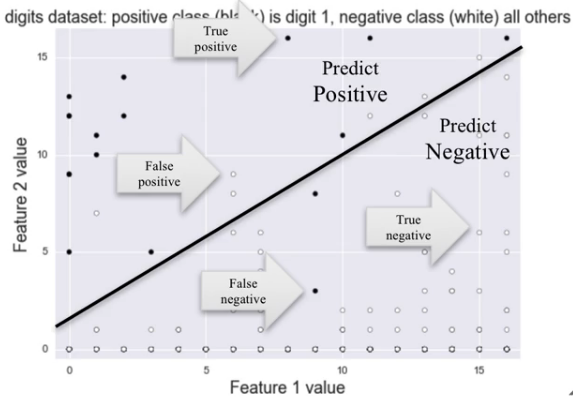
\includegraphics[width=\linewidth]{img/Diff-error-types-visualization.png} 
\end{center}

What I've done here is plot the data instances by using two specific feature values out of the total 64 feature values that make up each instance in the digits dataset. 

The black points here are the instances with true class positive namely the digit one and the white points have true class negative, that is, there are all the other digits except for one. The black line shows a hypothetical linear classifier's decision boundary for which any instance to the left of the decision boundary is predicted to be in the positive class and everything to the right of the decision boundary is predicted to be in the negative class. 

The true positive points are those black points in the positive prediction region and false positives are those white points in the positive prediction region. Likewise, true negatives are the white points in the negative prediction region and false negatives are black points in the negative prediction region. 

\subsection{Accuracy}

We've already seen one metric that can be derived from the confusion matrix counts namely \emph{Accuracy}. The successful predictions of the classifier, the ones where the predicted class matches the true class are along the \emph{diagonal} of the confusion matrix. 

$$Accuracy = \frac{TP + TN}{TP + TN + FP + FN}$$

\subsection{Classification Error}

But, let's look at some other evaluation metrics we can compute from these four numbers. Well, a very simple related number that's sometimes used is \emph{Classification Error}. Classification Error is equivalent to  one minus the accuracy.

$$Classification\ Error = \frac{FP + FN}{TP + TN + FP + FN}$$

$$Classification\ Error = 1 - Accuracy$$

\begin{center}
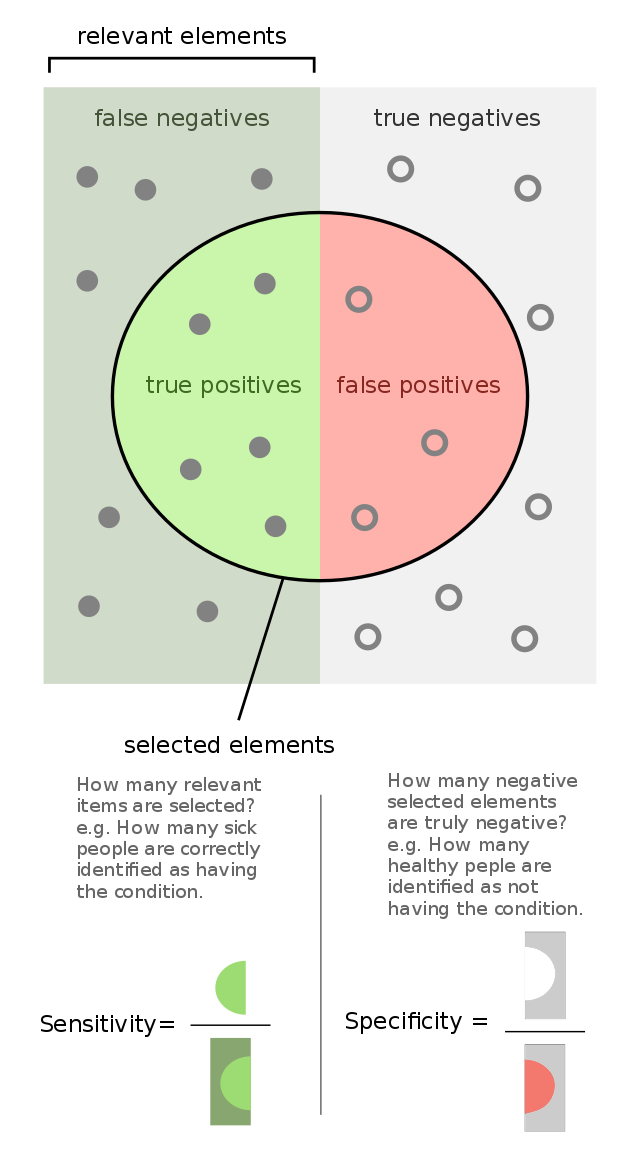
\includegraphics[width=\linewidth]{img/640px-Sensitivity-and-specificity.png} 
\end{center}

\subsection{Recall / True Positive Rate / Sensitivity}

Now, for a more interesting example, let's suppose, going back to our medical tumor detecting classifier that we wanted an evaluation metric that would give higher scores to classifiers that not only achieved the high number of \emph{true positives} but also \emph{avoided false negatives}. That is, that rarely failed to detect a true cancerous tumor. 

\emph{Recall}, also known as the \emph{True Positive Rate}, sensitivity or probability of detection~--- an evaluation metric. 

$$Recall = \frac{TP}{TP + FN}$$

What fraction of all positive instances does the classifier \emph{correctly} identify as positives?

You can see from this formula that there are two ways to get a larger recall number. First, by either increasing the number of true positives or by reducing the number of false negatives. Since this will make the denominator smaller. 

In this example there are 26 true positives and 17 false negatives which gives a recall of 0.6. 



\subsection{Precision}

Now suppose that we have a machine learning task, where it's really important to avoid false positives. In other words, we're fine with cases where not all true positive instances are detected but when the classifier does predict the positive class, we want to be very confident that it's correct. 

A lot of customer facing prediction problems are like this, for example, predicting when to show a user A query suggestion in a web search interface might be one such scenario. Users will often remember the failures of a machine learning prediction even when the majority of predictions are successes. 

So, precision is an evaluation metric that reflects the situation. 

$$Precision = \frac{TP}{TP + FP}$$

What fraction of positive predictions are correct?

So to increase precision, we must either increase the number of true positives the classifier predicts or reduce the number of errors where the classifier incorrectly predicts that a negative instance is in the positive class. 

Here, the classifier has made seven false positive errors and so the precision is 0.79. 

\subsection{False Positive Rate / Specificity}

Another related evaluation metric that will be useful is called the \emph{False Positive Rate}, also known as \emph{specificity}. This gives the fraction of all negative instances that the classifier incorrectly identifies as positive. 

$$False\ Positive\ Rate = \frac{TN}{TN + FP}$$

What fraction of all negative instances does the classifier \emph{incorrectly} identify as positives?

Here, we have seven false positives, which out of a total of 407 negative instances, gives a false positive rate of 0.02. 

Going back to our classifier visualization, let's look at how precision and recall can be interpreted. The numbers that are in the confusion matrix here are derived from this classification scenario. We can see that a precision of 0.68 means that about 68 percent of the points in the positive prediction region to the left of the decision boundary or 13 out of the 19 instances are correctly labeled as positive. A recall of 0.87 means, that of all true positive instances, so all black points in the figure, the positive prediction region has 'found about 87 percent of them' or 13 out of 15. 

If we wanted a classifier that was oriented towards higher levels of precision like in the search engine query suggestion task, we might want a decision boundary instead that look like this. Now, all the points in the positive prediction region seven out of seven are true positives, giving us a perfect precision of 1.0. 

\begin{center}
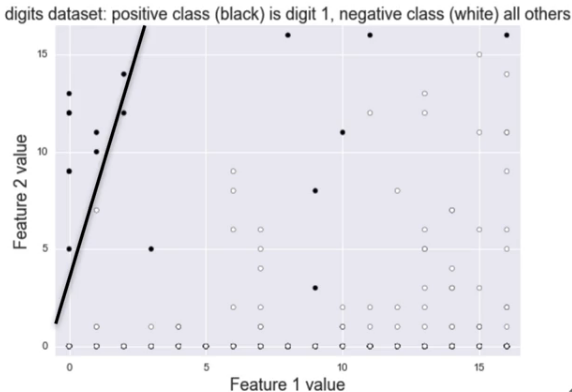
\includegraphics[width=\linewidth]{img/High-Precision-Lower-Recall.png} 
\end{center}

Now, this comes at a cost because out of the 15 total positive instances eight of them are now false negatives, in other words, they're incorrectly predicted as being negative. And so, recall drops to 7 divided by 15 or 0.47. 

On the other hand, if our classification task is like the tumor detection example, we want to minimize false negatives and obtain high recall. In which case, we would want the classifier's decision boundary to look more like this.

\begin{center}
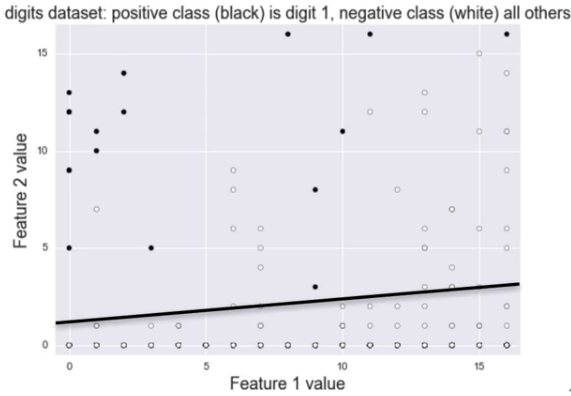
\includegraphics[width=\linewidth]{img/Low-Precision-High-Recall.png} 
\end{center}

 Now, all 15 positive instances have been correctly predicted as being in the positive class, which means these tumors have all been detected. 

However, this also comes with a cost since the number of false positives, things that the detector triggers as possible tumors for example that are actually not, has gone up. So, recall is a perfect 1.0 score but the precision has dropped to 15 out of 42 or 0.36. These examples illustrate a classic trade-off that often appears in machine learning applications. Namely, that you can often increase the precision of a classifier but the downside is that you may reduce recall, or you could increase the recall of a classifier at the cost of reducing precision. 

\emph{Recall oriented} machine learning tasks include medical and legal applications, where the consequences of not correctly identifying a positive example can be high. Often in these scenarios human experts are deployed to help filter out the false positives that almost inevitably increase with high recall applications. 

Many customer facing machine learning tasks, as I just mentioned, are often \emph{precision oriented} since here the consequences of false positives can be high, for example, hurting the customer's experience on a website by providing incorrect or unhelpful information. Examples include, search engine ranking and classifying documents to annotate them with topic tags. 

\subsection*{$F_1$ score and $F_\beta$ score}

When evaluating classifiers, it's often convenient to compute a quantity known as an $F_1$ score, that combines precision and recall into a single number. 

$$F_1 = 2 * \frac{Precision * Recall}{Precision + Recall}$$

$$F_1 = \frac{2*TP}{2*TP+FN+FP}$$

Mathematically, this is based on the harmonic mean of precision and recall using this formula. After a little bit of algebra, we can rewrite the $F_1$ score in terms of the quantities that we saw in the confusion matrix: true positives, false negatives and false positives. 

This $F_1$ score is a special case of a more general evaluation metric known as an $F_\beta$ score that introduces a parameter beta. 

$$F_\beta = (1+\beta^2) * \frac{Precision * Recall}{\beta^2*Precision + Recall}$$

$$F_\beta = \frac{(1+\beta^2)*TP}{(1+\beta^2)*TP+\beta * FN + FP}$$

By adjusting beta we can control how much emphasis an evaluation is given to precision versus recall. 

For example, if we have precision oriented users, we might say a beta equal to 0.5, since we want false positives to hurt performance more than false negatives. 

For recall oriented situations, we might set beta to a number larger than one, say two, to emphasize that false negatives should hurt performance more than false positives. 

The setting of beta equals one corresponds to the $F_1$ score special case that we just saw that weights precision and recall equally. 


\subsection{Metrics in Scikit-learn}

Let's take a look now at how we can compute these evaluation metrics in Python using scikit-learn. Scikit-learn provides functions \texttt{accuracy_score}, \texttt{precision_score}, \texttt{recall_score},  \texttt{f_score} and \texttt{fbeta_score}. The input to these functions is the same. The first argument \texttt{y_test} is the array of true labels of the test set data instances and the second argument is the array of predicted labels for the test set data instances. 

It's often useful when analyzing classifier performance to compute all of these metrics at once. So, sklearn metrics provides a handy \texttt{classification_report} function. Like the previous score functions, classification report takes the true and predicted labels as the first two required arguments. It also takes some optional arguments that control the format of the output. 

{\scriptsize
\begin{verbatim}
from sklearn.metrics import classification_report

print(classification_report(y_test, tree_predicted, 
      target_names=['not 1', '1']))
      
            precision recall f1-score support

       not 1     0.96   0.98     0.97     407
           1     0.79   0.60     0.68      43

   micro avg     0.95   0.95     0.95     450
   macro avg     0.87   0.79     0.83     450
weighted avg     0.94   0.95     0.94     450
\end{verbatim}
}

Here, we use the target names option to label the classes in the output table. The last column \texttt{support} shows the number of instances in the test set that have that true label. 

Here we show classification reports for four different classifiers on the binary digit classification problem. 
{\scriptsize
\begin{verbatim}
Random class-proportional (dummy)
               precision    recall  f1-score   support

       not 1       0.91      0.91      0.91       407
           1       0.12      0.12      0.12        43

   micro avg       0.83      0.83      0.83       450
   macro avg       0.51      0.51      0.51       450
weighted avg       0.83      0.83      0.83       450

SVM
               precision    recall  f1-score   support

       not 1       0.99      0.99      0.99       407
           1       0.88      0.88      0.88        43

   micro avg       0.98      0.98      0.98       450
   macro avg       0.94      0.94      0.94       450
weighted avg       0.98      0.98      0.98       450

Logistic regression
               precision    recall  f1-score   support

       not 1       0.99      0.99      0.99       407
           1       0.86      0.86      0.86        43

   micro avg       0.97      0.97      0.97       450
   macro avg       0.92      0.92      0.92       450
weighted avg       0.97      0.97      0.97       450

Decision tree
               precision    recall  f1-score   support

       not 1       0.96      0.98      0.97       407
           1       0.79      0.60      0.68        43

   micro avg       0.95      0.95      0.95       450
   macro avg       0.87      0.79      0.83       450
weighted avg       0.94      0.95      0.94       450
\end{verbatim}
}

The first set of results is from the dummy classifier and we can see that as expected both precision and recall for the positive class are very low since the dummy classifier is simply guessing randomly with low probability of predicting that positive class for the positive instances. 

\end{multicols}